\documentclass[11pt,answers]{exam}

% Load useful packages
% Read in necessary packages
\usepackage{import}
\usepackage{amsmath}
\usepackage{amsfonts}
\usepackage{amssymb}
\usepackage{graphicx}
\usepackage{hyperref}
\usepackage{color}
\usepackage{subfigure}
\usepackage{tikz}

% Set various options for exam package
\shadedsolutions % defines the style of the solution environment

% Set lesson name, etc.
\newcommand{\coursename}{Math 312}
\newcommand{\lessonname}{Problem Set 6}
\newcommand{\duedate}{5 April 2016}
\newcommand{\names}{Ian Gallmeister, Kevin Fortune, Alex Webb}

% Set headers/footers to look nice
\pagestyle{headandfoot}
\firstpageheader{\textbf{\large \coursename\ \lessonname}}{}{\textbf{\large Due \duedate}}
\firstpageheadrule
\runningheader{\textbf{\large \coursename\ \lessonname}}{}{\textbf{\large Due \duedate}}
\runningheadrule
\firstpagefooter{\names}{}{Page \thepage\ of \numpages}
\firstpagefootrule
\runningfooter{\names}{}{Page \thepage\ of \numpages}
\runningfootrule

% Define commands related to marking up content
\newcommand{\source}[1]{}

% Define commands related to general mathematical style
\renewcommand{\exp}[1]{e^{#1}}

\renewcommand{\theenumi}{(\textsc{\alph{enumi}})}
\renewcommand{\labelenumi}{\theenumi}
\renewcommand{\thequestion}{\arabic{question}}
\renewcommand{\questionlabel}{(\thequestion)}
%%%%%%%%%%%%%%%%%%%%%%%%%%%%%%%%%%%%%%%%%%%%%%%%%%%%%%%%%%%%

\begin{document}
\begin{questions}

\addtocounter{question}{35}
\item Find eigenvalues and eigenvectors for the following matrices (consider using a computer):
\begin{align*}
&\hbox{\textsc{(a)}} = \left(\begin{array}{ccc} 3 & -1 & 0 \\ -1 & 2 & -1 \\ 0 & -1 & 3 \end{array}\right)  &\hbox{\textsc{(b)}} = \left(\begin{array}{ccc} 1 & -3 & 11 \\ 2 & -6 & 16 \\ 1 & -3 & 7 \end{array}\right) \\ &\hbox{\textsc{(c)}} = \left(\begin{array}{ccc} -4 & -4 & 2 \\ 3 & 4 & -1 \\ -3 & -2 & 3 \end{array}\right)  &\textsc{(d)} = \left(\begin{array}{cccc} 4 & 0 & 0 & 0 \\ 1 & 3 & 0 & 0 \\ -1 & 1 & 2 & 0 \\ 1 & -1 & 1 & 1 \end{array}\right)
\end{align*}
\begin{solution}
Here, we used mathematica to solve this.  Each matrix got the commands:
\begin{verbatim}
M = Transpose[{{a,b,c},{d,e,f},{g,h,i}}]
MatrixForm[Transpose[Eigensystem[M]]]
\end{verbatim}
which gives us the a result in the form
\[
\left(\begin{array}{cc} \lambda_1 & \{v_{1,1}, v_{1,2}, v_{1,3}\} \\ \lambda_2 & \{v_{2,1}, v_{2,2}, v_{2,3}\} \\ \lambda_3 & \{v_{3,1}, v_{3,2}, v_{3,3}\}  \end{array}\right)
\]
As such, we find that

\begin{align*}
&\hbox{\textsc{(a)}} \Rightarrow &\lambda_1 = 4, \vec{v}_2 = \left(\begin{array}{c}1\\-1\\1\end{array}\right) & &\lambda_2 = 3, \vec{v}_2 = \left(\begin{array}{c}-1\\0\\1\end{array}\right) & &\lambda_3 = 1, \vec{v}_3 = \left(\begin{array}{c}1\\2\\1\end{array}\right) \\
&\hbox{\textsc{(b)}} \Rightarrow &\lambda_1 = 1 + i, \vec{v}_1 = \left(\begin{array}{c} 3 - 2i \\ 3 - i \\ 1 \end{array}\right) & &\lambda_2 = 1 - i, \vec{v}_2 = \left(\begin{array}{c} 3 + 2i \\ 3 + i \\ 1 \end{array}\right) & &\lambda_3 = 0, \vec{v}_3 = \left(\begin{array}{c} 3 \\ 1 \\ 0 \end{array}\right) \\
&\hbox{\textsc{(c)}} \Rightarrow &\lambda_{1} = 1, \vec{v}_1 = \left(\begin{array}{c} 1 \\ 0 \\ 3 \end{array}\right), & &\lambda_{1} = 1, \vec{v}_2 = \left(\begin{array}{c} -2 \\ 0 \\ 3 \end{array}\right) & &\lambda_3 = -1, \vec{v} = \left(\begin{array}{c} 2 \\ -1 \\ 1 \end{array}\right)
\end{align*}
\[
\hbox{\textsc{(d)}} \Rightarrow \:\: \lambda_1 = 1, \vec{v}_1 = \left(\begin{array}{c} 0 \\ 0 \\ 0 \\ 1\end{array}\right) \:\: \lambda_2 = 2, \vec{v}_2 = \left(\begin{array}{c} 0 \\ 0 \\ 1 \\ 1\end{array}\right) \:\: \lambda_3 = 3, \vec{v}_3 = \left(\begin{array}{c} 0 \\ 1 \\ 1 \\ 0\end{array}\right) \:\: \lambda_4 = 4, \vec{v}_4 = \left(\begin{array}{c} 1 \\ 1 \\ 0 \\ 0\end{array}\right)
\]
\end{solution}

\pagebreak
\item a) Find the explicit formula for the characteristic polynomial $det(A-\lambda) = -\lambda^3 +a\lambda^2 - b\lambda + c$ of a general 3x3 matrix. Verify that a = tr(A), c = det(A). What is the formula for b?

\begin{solution}
For a 3x3 matrix 
\[
\hbox{\hfill\textsc{(c)}} = \left(\begin{array}{ccc} A_{11} & A_{12} & A_{13}  \\ A_{21} & A_{22} & A_{23}  \\ A_{31} & A_{32} & A_{33}  \end{array}\right)
\]

The $ =$ 
\begin{multline*}
\det(A - \lambda I) = (A_{11} - \lambda)((A_{22}- \lambda)(A_{33}- \lambda) \\- A_{23}A_{32}) - (A_{12} - \lambda)(A_{21}(A_{33}- \lambda) - A_{23}A_{31}) - (A_{13} - \lambda)(A_{21}A_{32} - (A_{22}- \lambda)A_{31})
\end{multline*}
We can see that if we multiply this out, we will be able to regroup all terms as coefficients of $\lambda^3,\lambda^2,\lambda^1$, and $\lambda^0$. After expanding and regrouping the coefficients, we find:
\begin{equation*}
a = A_{11} + A_{22} +A_{33} \\
\end{equation*}
\begin{equation*}
b = -(A_{11}A_{22}-A_{11}A_{33}+A_{22}A_{33}-A_{23}A_{32}-A_{12}A_{21}-A_{13}A_{31})
\end{equation*}
\begin{equation*}
c = (A_{11})((A_{22})(A_{33}) - A_{23}A_{32}) - (A_{12})(A_{21}(A_{33}) - A_{23}A_{31}) - (A_{13} )(A_{21}A_{32} - (A_{22})A_{31})
\end{equation*}
\end{solution}

b) Prove that if A has eigenvalues $\lambda_1,\lambda_2, \lambda_3$, then a = tr(A)  = $\lambda_1 + \lambda_2 + \lambda_3$, b = $\lambda_1\lambda_2 + \lambda_1\lambda_3 + \lambda_2\lambda_3$, c = det(A) = $\lambda_1\lambda_2\lambda_3$

\begin{solution}
Let $\Lambda$ be the 3x3 diagonal matrix with the eigenvalues of A along the diagonal. We know there exists a matrix $S$ where
\begin{equation}
S^{-1}AS = \Lambda
\end{equation}
and therefore 
\begin{equation}
tr(S^{-1}AS) = tr(\Lambda)
\end{equation}
we can rewrite the left side as
\begin{equation}
tr((S^{-1}A)S)
\end{equation}
\begin{equation}
tr(S(S^{-1}A))
\end{equation}
\begin{equation}
tr((SS^{-1})A)
\end{equation}
\begin{equation}
tr((I)A) = tr(A)
\end{equation}
We know the trace of $\Lambda$ is the sum of its diagonal elements $\lambda_1,\lambda_2,\lambda_3$, so 
\begin{equation}
tr(A) = tr(\Lambda) = \lambda_1+\lambda_2+\lambda_3
\end{equation}
To show that $det(A) = \lambda_1\lambda_2\lambda_3$, we need to know that the determinant of a diagonal matrix $\Lambda$ is the product of its diagonal elements, $\lambda_1,\lambda_2,\lambda_3$. Using a similar process to the proof for tr(A), we find
\begin{equation}
det(A) = det(\Lambda) = \lambda_1\lambda_2\lambda_3
\end{equation}
\end{solution}

\item Diagonalization.
\begin{solution}
Using Wolfram Alpha, we found we can write A as $A = S\Lambda S^{-1}$ where 
\[
S = \left(\begin{array}{cc}\frac{-3}{5} - \frac{i}{5} & \frac{-3}{5} + \frac{i}{5}\\1 & 1\end{array}\right), \hbox{\hspace{1.5em}} \Lambda = \left(\begin{array}{cc}-1 - i & 0\\0 & -1 + i \end{array}\right), \hbox{\hspace{1.5em}} S^{-1} = \left(\begin{array}{cc} \frac{5i}{2} & \frac{1}{2} + \frac{3i}{2} \\   -\frac{5i}{2} & \frac{1}{2} - \frac{3i}{2} \end{array}\right)
\]

To find $A = TRT^{-1}$, we first rewrote the eigenvectors in the form
\begin{equation}
v_{1,2} = \hbox{\hspace{1.5em}} \left(\begin{array}{c} -3 \\ 5 \end{array}\right) \pm i\hbox{\hspace{1.5em}} \left(\begin{array}{c} 1 \\ 0 \end{array}\right)
\end{equation}
This gave us the information we needed to construct T. So, we found $T, R,$ and $T^{-1}$ to be
\[
T = \left(\begin{array}{cc}-3 & 1 \\5 & 0\end{array}\right), \hbox{\hspace{1.5em}} R = \left(\begin{array}{cc}-1 & 1 \\-1 & -1 \end{array}\right), \hbox{\hspace{1.5em}} T^{-1} = \left(\begin{array}{cc} 0 & \frac{1}{5}  \\  1 & \frac{3}{5} \end{array}\right)
\]
\end{solution}

\item Diagonalize these matrices.  Write them in the form $A = S\Lambda S^{-1}$
\[
\hbox{\textsc{(a)}} = \left(\begin{array}{ccc}8 & 0 & -3 \\ -3 & 0 & -1 \\ 3 & 0 & -2 \end{array}\right) 
\hbox{\hfill\textsc{(b)}} = \left(\begin{array}{ccc} 2 & 5 & 5 \\ 0 & 2 & 0 \\ 0 & -5 & -3 \end{array} \right)
\hbox{\hfill\textsc{(c)}} = \left(\begin{array}{cccc} 2 & 1 & -1 & 0 \\ -3 & -2 & 0 & 1 \\ 0 & 0 & 1 & -2 \\ 0 & 0 &t 1 & -1 \end{array}\right)
\]

\begin{solution}
Using the \texttt{Eigensystem[]} and \texttt{Inverse[]} functions in Mathematica, we find that:
\begin{align*}
\hbox{\textsc{(a)}} \:\:\:\: &\left(\begin{array}{ccc}8 & 0 & -3 \\ -3 & 0 & -1 \\ 3 & 0 & -2 \end{array}\right) \hbox{has a non-invertible $S \Rightarrow$ nondiagonizable}\\
\hbox{\textsc{(b)}} \:\:\:\: &\left(\begin{array}{ccc} 2 & 5 & 5 \\ 0 & 2 & 0 \\ 0 & -5 & -3 \end{array} \right) = \left(\begin{array}{ccc} -1 & 0 & 1 \\ 0 & -1 & 0 \\ 1 & 1 & 0 \end{array}\right)
\left(\begin{array}{ccc} -3 & 0 & 0 \\ 0 & 2 & 0 \\ 0 & 0 & 2 \end{array}\right)
\left(\begin{array}{ccc} 0 & 1 & 1 \\ 0 & -1 & 0 \\ 1 & 1 & 1 \end{array}\right)\\
\hbox{\textsc{(c)}} \:\:\:\: &\left(\begin{array}{cccc} 2 & 1 & -1 & 0 \\ -3 & -2 & 0 & 1 \\ 0 & 0 & 1 & -2 \\ 0 & 0 & 1 & -1 \end{array}\right) = 
\left(\begin{array}{cccc} 1 & -1 & -1 & 3 \\ 0 & 3 & 1 & -4 \\ 3 & 0 & 0 & 2 \\ 3 & 0 & 0 & 1 \\ \end{array}\right)
\left(\begin{array}{cccc} -1 & 0 & 0 & 0 \\ 0 & -1 & 0 & 0 \\ 0 & 0 & 1 & 0 \\ 0 & 0 & 0 & 0 \\ \end{array} \right) 
\left(\begin{array}{cccc} 0 & 0 & -\frac{1}{3} & \frac{2}{3} \\ \frac{1}{2} & \frac{1}{2} & \frac{2}{3} & -\frac{5}{6} \\ -\frac{3}{2} & -\frac{1}{2} & 2 & -\frac{3}{2} \\ 0 & 0 & 1 & -1 \\\end{array}\right)
\end{align*}
\end{solution}

\item Consider the differential equation
\[
\dddot{u} + \ddot{u} + \dot{u} + u = 0
\]
\begin{enumerate}
\item Solve the equation by writing it as a dynamical system in standard form and using a linear algebra based method. Make sure to write your final solution in terms of real quantities only.

\begin{solution}
First, setup a system of equations in standard form:

$$x_1 = x$$
$$x_2 = \dot{x_1}$$
$$x_3 = \dot{x_2}$$
$$\dot{x_3} = -x_3 - x_2 - x_1$$

Second, write the system of equations as the product of a matrix and vector:

$$\dot{X} = \left(\begin{array}{ccc} \dot{x_1} \\ \dot{x_2} \\ \dot{x_3} \end{array}\right)$$
$$X = \left(\begin{array}{ccc} {x_1} \\ {x_2} \\ {x_3} \end{array}\right)$$
$$A = \left(\begin{array}{ccc} 0 & 1 & 0 \\ 0 & 0 & 1 \\ -1 & -1 & -1 \end{array}\right)$$

Third, I used Mathematica to find the eigenvalues and eigenvectors of the matrix. They are:

$$\lambda_1 = -1 $$
$$\lambda_2 = i$$
$$\lambda_3 = -i$$

$$v_1 = \left(\begin{array}{ccc} 1 \\ -1 \\ 1 \end{array}\right) $$
$$v_2 = \left(\begin{array}{ccc} -1 \\ -i \\ 1 \end{array}\right)$$
$$v_3 = \left(\begin{array}{ccc} -1 \\ i \\ 1 \end{array}\right)$$

This gives us the general solution:

$$X = c_1\left(\begin{array}{ccc} 1 \\ -1 \\ 1 \end{array}\right)e^{-t} + C_2\left(\begin{array}{ccc} -1 \\ -i \\ 1 \end{array}\right)e^{it} + c_3\left(\begin{array}{ccc} -1 \\ i \\ 1 \end{array}\right)e^{-it}$$

\end{solution}

\item Solve the equation with the ansatz $u = e^{\lambda t}$, finding all valid $\lambda$, and taking a linear combination of those solutions.  Make sure to write your solution in terms of real quantities only.

\begin{solution}

Begin with the characteristic equation:

$$\lambda^3 + \lambda^2 + \lambda + 1 = 0$$

$$\lambda = -1,i,-i$$

I solved the polynomial using Wolfram-Alpha. Note that these are the same as the eigenvalues in part A. These give us the general solution:

$$x = C_1e^{-t} + C_2e^{it} + C_3e^{-it}$$

Each term is linearly independant. 

\end{solution}

\end{enumerate}


\item Consider the initial value problem
\begin{align*}
\dot{x}_1 &= 2x_1 + 4x_2 - 4x_4 \\
\dot{x}_2 &= 3x_1 - 2x_3 - x_4\\
\dot{x}_3 &= x_3 \\
\dot{x}_4 &= 3x_1 + 2x_2 - 2x_3 - 3x_4
\end{align*}
and the initial conditions $x_1(0) = 3, x_2(0) = 1, x_3(0) = 2, x_4(0) = 4$
\begin{enumerate}
\item Write the initial value problem in matrix form.
\item Find the exact solution to the problem.
\item The solution simplifies in the long-time limit. Explain how, and discuss the long-term behavior.
\end{enumerate}

\begin{solution}
A) Initial Value problem:
\[
\dot{x} = Ax, \hbox{\hspace{1.5em}} x = \left(\begin{array}{c}x_1 \\ x_2 \\ x_3 \\ x_4\end{array}\right), \hbox{\hspace{1.5em}} x_0 = \left(\begin{array}{c}3 \\ 1 \\ 2 \\ 4\end{array}\right), \hbox{\hspace{1.5em}} A = \left(\begin{array}{cccc} 2 & 4 & 0 & -4 \\  3 & 0 & -2 & -1 \\  0 & 0 & 1 & 0\\3 & 2 & -2 & 3  \end{array}\right)
\]
B) To find the exact solution, we first used the following code in Mathematica:
\begin{verbatim}
xdot = {{x1dot}, {x2dot}, {x3dot}, {x4dot}};
x = {{x1}, {x2}, {x3}, {x4}};
A = {{2, 4, 0, -4}, {3, 0, -2, -1}, {0, 0, 1, 0}, {3, 2, -2, -3}};
MatrixForm[A]
(*xdot=Ax*)
MatrixForm[Transpose[Eigensystem[A]]]
\end{verbatim}
This gave us the eigenvalues $\lambda_{1,2,3,4} = -2,2,-1,1$, and the corresponding eigenvectors 
\[
\hbox{\hspace{1.5em}} v_1 = \left(\begin{array}{c}-1\\ 2 \\ 0 \\ 1\end{array}\right), \hbox{\hspace{1.5em}} v_2 = \left(\begin{array}{c}1 \\ 1 \\ 0 \\ 1\end{array}\right), \hbox{\hspace{1.5em}} v_3 = \left(\begin{array}{c}0 \\ 1 \\ 0 \\ 1\end{array}\right), \hbox{\hspace{1.5em}} v_4 = \left(\begin{array}{c}0 \\ 1 \\ -1 \\ 1\end{array}\right)
\]
So now we can build the exact solution:
\[
x = C_1\left(\begin{array}{c}-1\\ 2 \\ 0 \\ 1\end{array}\right) e^{-2t}+ C_2 \left(\begin{array}{c}1 \\ 1 \\ 0 \\ 1\end{array}\right)e^{2t} + C_3\left(\begin{array}{c}0 \\ 1 \\ 0 \\ 1\end{array}\right)e^{-t} + C_4\left(\begin{array}{c}0 \\ 1 \\ -1 \\ 1\end{array}\right)e^{t}
\]
Now we can find the values for our constants.  Plugging in our values for $x_0$ gives us the equations:
\begin{align*}
3 &= -C_1 + C_2 \\
1 &= 2C_1 + C_2 + C_3 + C_4 \\
2 &= -C_4 \\
4 &= C_1 + C_2 + C_3 + C_4
\end{align*}
From that, we find that $C_1 = -3, ~ C_2 = 0, ~ C_3 = 9\hbox{, and } C_4 = -2$ so
\[
x =
-3\left(\begin{array}{c}-1\\ 2 \\ 0 \\ 1\end{array}\right) e^{-2t} + 
9\left(\begin{array}{c}0 \\ 1 \\ 0 \\ 1\end{array}\right)e^{-t} - 
2\left(\begin{array}{c}0 \\ 1 \\ -1 \\ 1\end{array}\right)e^{t}
\]
\newline\textsc{(c)} As $t$ goes to infinity, the terms with negative exponents approach zero, leaving us with a single exponential term:
\[
x = -2\left(\begin{array}{c}0 \\ 1 \\ -1 \\ 1\end{array}\right)e^{t}
\]
\end{solution}
\item Consider the initial value problem
\begin{align*}
\dot{x_1} &= 2x_1 + 4x_2 + 4x_3\\
\dot{x_2} &= x_1 + 2x+2 + 3x+3\\
\dot{x_3} &= -3x_1 -4x_2 - 5x_3\\
\end{align*}
\begin{enumerate}
\item Write the initial value problem in matrix form.
\item Find the exact solution to the problem.
\item If your exact solution in part \textsc{(b)} is written in terms of complex quantities, rewrite it to be in a form that only has real quantities.
\item The solution simplifies in the long-time limit. Explain how, and discuss the long-term behavior.
\item Using Matlab or another program of your choice, make a 3-d plot of the analytical solution, that is, a plot of the trajectory in the 3-d phase space. (Do NOT solve the equations numerically, e.g., using Matlab). Explain/interpret what you see in your plot light of your answers to the previous parts of this problem.
\end{enumerate}

\begin{solution}
\begin{enumerate}
\item The IVP in matrix form is:
\[
\dot{x} = Ax, \hbox{\hspace{1.5em}} x = \left(\begin{array}{c}x_1 \\ x_2 \\ x_3\end{array}\right), \hbox{\hspace{1.5em}} x_0 = \left(\begin{array}{c}2 \\ 4 \\ 5\end{array}\right), \hbox{\hspace{1.5em}} A = \left(\begin{array}{ccc} 2 & 4 & 4 \\ 1 & 2 & 3 \\ -3 & -4 & -5 \end{array}\right)
\]
\item To find the exact solution, use \texttt{MatrxForm[Transpose[Eigensystem[]]]} to find:
\newline $\displaystyle \left(\begin{array}{cc} 2i & \{-2, -1-i, 2\} \\ -2i & \{ -2, -1 + i, 2 \} \\ -1 & \{ 0, -1, 1 \} \end{array}\right)$ so 
\[
x = C_1 e^{2it}\left(\begin{array}{c}-2 \\ -1-i \\ 2\end{array}\right) + C_2e^{-2it}\left(\begin{array}{c} -2 \\ -1 + i \\ 2 \end{array}\right) + C_3e^{-t}\left(\begin{array}{c}0 \\ -1 \\ 1\end{array}\right)
\]
Now we can use \texttt{Solve[\{\{2\}, \{4\}, \{5\}\} == C1*\{\{-2\}, \{-1 - I\}, \{2\}\} + C2*\{\{-2\}, \{-1 + I\}, \{2\}\} + C3*\{\{0\}, \{-1\}, \{1\}\}, \{f, g, h\}]} to find that $C_1 = -1/2 + 5i$, $C_2 = -1/2 - 5i$, and $C_3 = 7$.  Thus,
\[
x = \left(-1/2 + 5i\right) e^{2it}\left(\begin{array}{c}-2 \\ -1-i \\ 2\end{array}\right) + \left( -1/2 - 5i \right)e^{-2it}\left(\begin{array}{c} -2 \\ -1 + i \\ 2 \end{array}\right) + 7e^{-t}\left(\begin{array}{c}0 \\ -1 \\ 1\end{array}\right)
\]
\item To write in completely real terms, we define our solution $x$ in Mathematica, and use \texttt{MatrixForm[Simplify[x]]} to find that $x = $
\[
\left(\begin{array}{c} 2 (\cos (2 t)+10 \sin (2 t)) \\ -7 e^{-t}+11 \cos (2 t)+9 \sin (2 t) \\ 7 e^{-t}-2 \cos (2 t)-20 \sin (2 t) \end{array}\right) = \cos{2t}\left(\begin{array}{c}2 \\ 11 \\ -2\end{array}\right) + \sin{2t}\left(\begin{array}{c}10 \\ 9 \\ -20 \end{array}\right) + e^{-t}\left(\begin{array}{c}0 \\ -7 \\ 7\end{array}\right)
\]
\item  As one can see, there is an exponential term which will go to zero as $t \to \infty$, so eventually, this will be a 2D cycle in a plane - a quickly collapsing spiral in 3D space.
\item Here, we see three views of the solution $x$.  As one can see, there is some vertical motion in the $e^{-t}$ direction which quickly becomes an elliptical path embedded in a plane of the space.  There is also a perspective from which the path just seems to be an ellipse.  This is the angle of the $\sin$-$\cos$ plane.
\newline
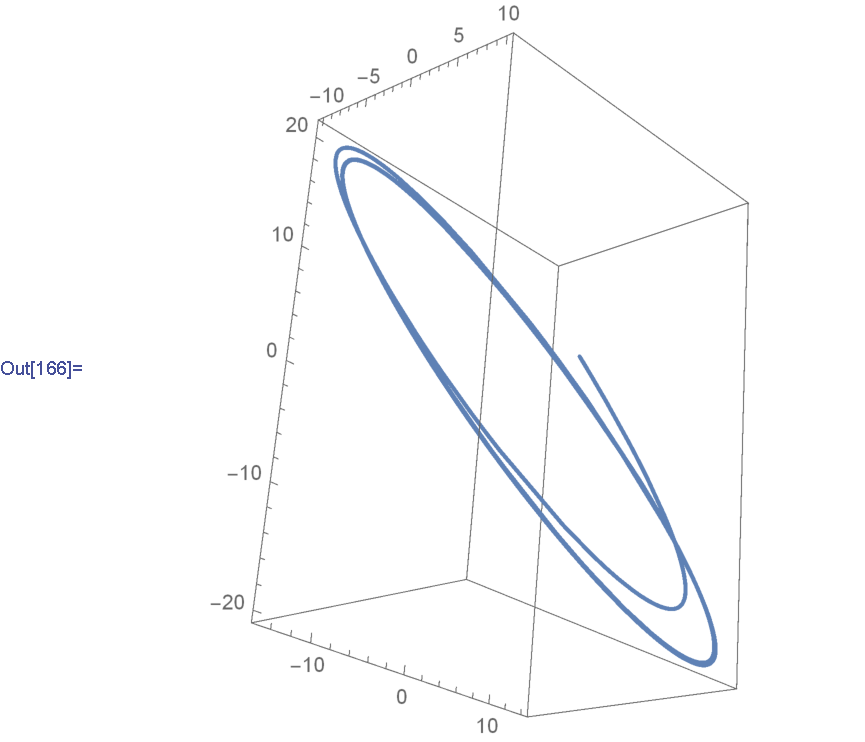
\includegraphics[width=0.3\textwidth]{p42plot.pdf}
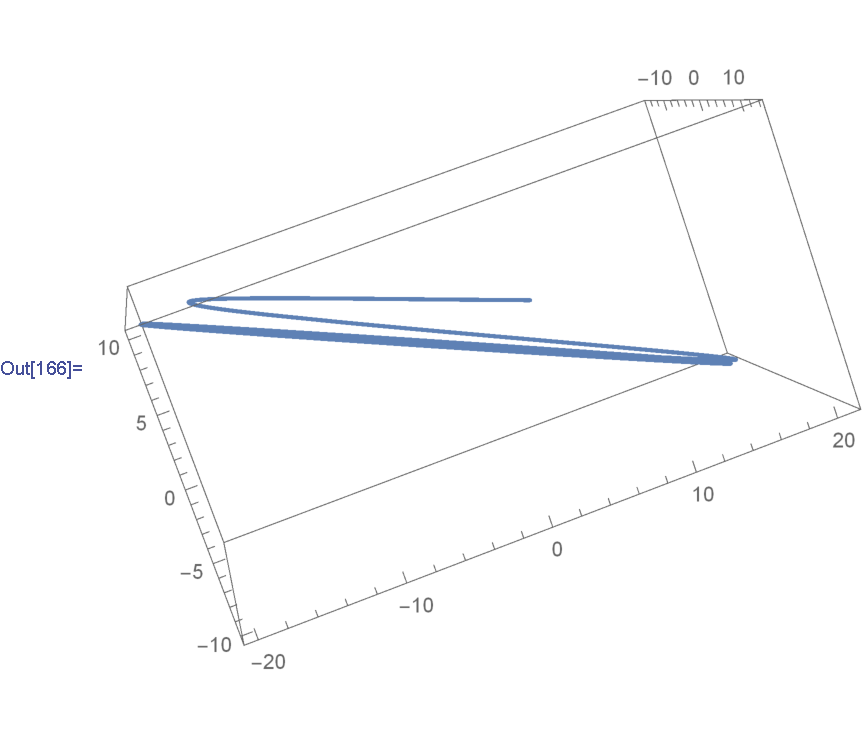
\includegraphics[width=0.3\textwidth]{p42plot2}
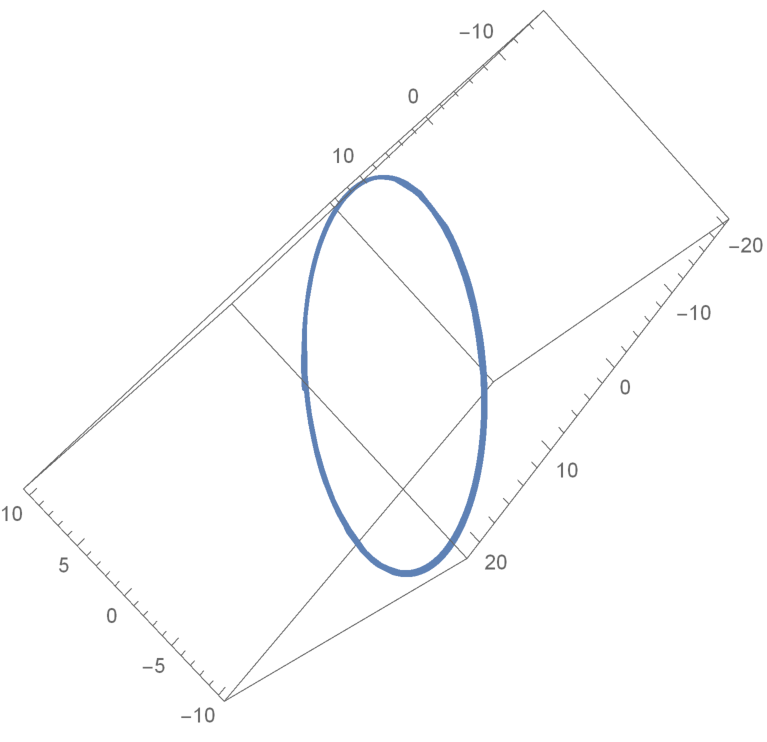
\includegraphics[width=0.27\textwidth]{p42plot3}
\end{enumerate}
\end{solution}



\end{questions}
\end{document}